%-*- mode: LaTeX; -*-

%Consists of Si and C atoms, crystal. (Arranged periodically)
%There exists many (Citation?) different kinds of polytypes
%Polytypes can be thought of as stacking sequence of hexagonal layers
%Base is one C and one Si
%Si and C faces, what is that?
%If I do anything on bulk, then I should discuss planes here. (Since the goal is to have (100) plane).

%The atoms are bonded together by X bonds.
%The band structure is shown...
%Indirect band gap of...

%Some relevant properties
%Mobility
%Dielectric constant

%Nitrogen as background doping
%Possible acceptors are
%Boron doping gives good band diagram as seen...


\chapter{An introduction to silicon carbide}
\label{sec:sic}
This chapter describes the relevant properties of SiC. Section \ref{sec:crystal_structure} describes the atomic arrangement in the material, and some different arrangements are discussed. Section \ref{sec:band_structure} discusses the energy band structure of 3C-SiC. Finally section \ref{sec:doping_in_3C} describes the mechanism and some effects of doping in 3C-SiC. 

\section{Crystal structure}
\label{sec:crystal_structure}
Silicon carbide is a crystalline material consisting of silicon and carbon atoms. The crystalline nature of the material means that the atoms are arranged in a periodically repeating structure called a \emph{lattice}. For given chemical elements there may be several different ways to arrange the atoms in a lattice, i.e. different chemical compounds of the same types of atoms. This is called \emph{polytypism}, where the different lattice structures are called \emph{polytypes} of the material. SiC has a large number of different polytypes. There are more than 250 known polytypes of SiC \cite{Cheung2006}. The different polytypes can be described as different stacking orders of hexagonal layers of atoms \cite{Mirgorodsky1995}. 


\begin{figure}
\begin{center}
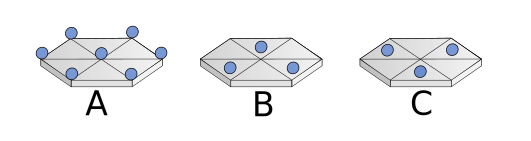
\includegraphics[scale=0.9]{hex5.pdf}
\caption{Hexagonal layer structure
\label{fig:hex}}
\end{center}
\end{figure}


\section{Band structure}
\label{sec:band_structure}

%\section{Some properties}
%\label{sec:}

\section{Doping in 3C}
\label{sec:doping_in_3C}

